\documentclass[12pt, fleqn, openany]{studyGuide}
\setstretch{1.4}
\enableInlineReview
\renewcommand{\VMBookTitle}{Audit Review}
\renewcommand{\VMBookSubtitle}{Grade 7 --- Ch Graphic Review --- Changed Questions}
\renewcommand{\VMFooterURL}{https://viewmath.com/grade7}
\renewcommand{\VMFooterURLDisplay}{ViewMath.com/Grade7}
\begin{document}

\begin{center}
\begin{tcolorbox}[
	enhanced,
	colback=white,
	colframe=funTeal!60,
	boxrule=1.5pt,
	arc=10pt,
	outer arc=10pt,
	width=0.9\linewidth,
	halign=center,
	top=5mm, bottom=5mm,
]
	{\Large\bfseries\sffamily\color{funTealDark}Audit Review}\\[2mm]
	{\large\sffamily\color{funGrayDark}Grade 7 --- Ch Graphic Review --- Changed Questions}\\[2mm]
	{\normalsize\sffamily\color{funGrayDark}Verify corrections below}
\end{tcolorbox}
\end{center}

\newpage
\section*{3-9-q23 \hfill \normalsize\texttt{tests\_questions\_bank\_2/topics\_additional/ch03-09-introduction-to-square-roots.tex}}
\begin{practiceQuestion}{3-9-q23}{gmc}
\begin{questionText}
The diagram shows a square with area $A$. What is the side length?

\begin{center}
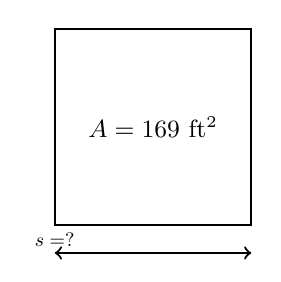
\begin{tikzpicture}[scale=0.78]
  \draw[thick] (0,0) rectangle (3.2,3.2);
  \node[font=\small] at (1.6,1.6) {$A = 169$ ft$^2$};
  \draw[thick,<->] (0,-0.45) -- (3.2,-0.45);
  \node[midway,below,font=\small] at (1.6,-0.45) {$s = ?$};
\end{tikzpicture}
\end{center}
\end{questionText}
\choiceA{$11$ ft}
\choiceB{$12$ ft}
\choiceC{$13$ ft}
\choiceD{$14$ ft}
\correctAnswer{C}
\explanation{$s = \sqrt{169} = 13$ ft. Because $13 \times 13 = 169$.}
\end{practiceQuestion}

\newpage
\section*{3-9-q25 \hfill \normalsize\texttt{tests\_questions\_bank\_2/topics\_additional/ch03-09-introduction-to-square-roots.tex}}
\begin{practiceQuestion}{3-9-q25}{gsa}
\begin{questionText}
The diagram shows two squares. What is the total area?

\begin{center}
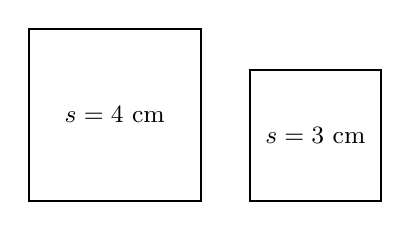
\begin{tikzpicture}[scale=0.52]
  \draw[thick] (0,0) rectangle (4.2,4.2);
  \node[font=\small] at (2.1,2.1) {$s = 4$ cm};
  \draw[thick] (5.4,0) rectangle (8.6,3.2);
  \node[font=\small] at (7.0,1.6) {$s = 3$ cm};
\end{tikzpicture}
\end{center}
\end{questionText}
\correctAnswer{$25$ cm$^2$}
\explanation{Area $1$: $4^2 = 16$ cm$^2$. Area $2$: $3^2 = 9$ cm$^2$. Total: $16 + 9 = 25$ cm$^2$.}
\end{practiceQuestion}

\newpage
\section*{3-9-q26 \hfill \normalsize\texttt{tests\_questions\_bank\_2/topics\_additional/ch03-09-introduction-to-square-roots.tex}}
\begin{practiceQuestion}{3-9-q26}{gsa}
\begin{questionText}
Use the number line to estimate $\sqrt{45}$ to the nearest tenth.

\begin{center}
\begin{tikzpicture}[scale=1.05]
  \draw[thick,->] (5.5,0) -- (8.5,0);
  \foreach \x in {6,7,8} \draw (\x,0.1) -- (\x,-0.1) node[below,font=\small] {$\x$};
  \foreach \x in {6.1,6.2,...,7.9} \draw (\x,0.05) -- (\x,-0.05);
  \node[above left,font=\small] at (6.12,0.08) {$\sqrt{36}$};
  \node[above right,font=\small] at (6.88,0.08) {$\sqrt{49}$};
  \fill[funBlue] (6.7,0) circle (0.1);
  \node[above,font=\small,funBlue] at (6.7,0.38) {$\sqrt{45} \approx ?$};
\end{tikzpicture}
\end{center}
\end{questionText}
\correctAnswer{$\approx 6.7$}
\explanation{$6^2 = 36$ and $7^2 = 49$. $45$ is $\dfrac{9}{13}$ of the way from $36$ to $49$, about $0.69$. So $\sqrt{45} \approx 6.7$.}
\end{practiceQuestion}

\newpage
\section*{3-11-q26 \hfill \normalsize\texttt{tests\_questions\_bank\_2/topics\_additional/ch03-11-introduction-to-scientific-notation.tex}}
\begin{practiceQuestion}{3-11-q26}{gsa}
\begin{questionText}
The bar graph compares masses of objects in scientific notation. About how many times heavier is Object B than Object A?

\begin{center}
\begin{tikzpicture}[xscale=0.7,yscale=0.55]
  \draw[thick,->] (0,0) -- (0,6);
  \draw[thick,->] (0,0) -- (5,0);
  \node[font=\small,rotate=90] at (-1.0,3) {Mass (kg)};
  \draw (-0.1,2) -- (0.1,2);
  \draw (-0.1,5) -- (0.1,5);
  \node[left,font=\small] at (-0.18,2) {$10^2$};
  \node[left,font=\small] at (-0.18,5) {$10^5$};
  \fill[funBlue] (1,0) rectangle (2,2);
  \fill[funGreen] (3,0) rectangle (4,5);
  \node[below,font=\small] at (1.5,-0.18) {A};
  \node[below,font=\small] at (3.5,-0.18) {B};
\end{tikzpicture}
\end{center}
\end{questionText}
\correctAnswer{$1{,}000$ times heavier}
\explanation{$\dfrac{10^5}{10^2} = 10^3 = 1{,}000$. Object B is $1{,}000$ times heavier than Object A.}
\end{practiceQuestion}

\end{document}